\section{}
\subsection{Exercise 1 (Perfect secrecy.)}
We define the following encryption scheme for messages, keys and
ciphertexts in $\mathbb{Z}_n$, where $\mathbb{Z}_n$ is essentially 
the integers in the interval $[0,n[$ 
(in fact $(\mathbb{Z}_n,+)$ forms a group):
\smallskip
\begin{itemize}
  \item $\Gen$ outputs a key $k \in \K$ selected uniformly at random.
  \item $\Enc_k(m) := k+m \mod n$
  \item $\Dec_k(c) := c-k \mod n$
\end{itemize}
\smallskip
Suppose messages are drawn from $\M$ according to the binomial
distribution. More precisely $M\sim \mathrm{Bi}(n-1,p)$ for some probability $p$ 
which means that $\forall m\in \M: \Pr[M=m]=\binom{n-1}{m}p^{m}(1-p)^{n-1-m}$.
\smallskip
\begin{enumerate}
  \item Show that the encryption scheme above is perfectly secret.
  \item Evaluate $\Pr[C=c]$ for every $c \in \C$.
  \item Evaluate $\Pr[K=k|C=c]$ for every $k\in \K$ and $c\in \C$. 
\end{enumerate}

\begin{solution}
  \begin{enumerate}
    \item
      We have secret privacy if : $Pr[C = c | M = m_0] = Pr[C = c | M = m_1] $ for every $m_0, m_1 \in \M$ and $c \in \C$.
      
      Let $c \in \C$ and $m\in \M$.
      We have :
      \begin{align*}
        \Pr[C = c | M = m]
        & = \Pr[M + K = c \pmod{n} | M = m]\\
        & = \Pr[m + K = c \pmod{n}]\\
        & = \Pr[m + K = c \pmod{n}]\\
        & = \Pr[K = c - m \pmod{n}]\\
        & = \frac{1}{n} \text{ (because k is selected \textbf{uniformly at random} in } \K \text{ where } |\K| = n )\\
        & = \Pr[C = c | M = m'] \text{ for every } m' \in \M
      \end{align*}
      Therefore, we have :
      \[
        \Pr[C = c | M = m_1] = \Pr[C = c | M = m_2]
      \]
      for every $c \in \C$ and $m_1,m_2 \in \M$. \\
      Which means we have perfect secrecy.
    \item
        Using the the result obtained at last exercice and the equivalent definitions about private secrecy, we can obtain :
      \begin{align*}
          \Pr[C = c]  & = \Pr[C = c | M = m] \text{ for every } m \in \M \\
          & = \frac{1}{n}
      \end{align*}
      Other way to solve it (thanks to Benoît Legat) : 
      \begin{align*}
        \Pr[C = c]
        & = \sum_{m \in \M} \Pr[\Enc_k(M) = c | M = m] \Pr[M = m]\\
        & = \frac{1}{n} \sum_{m \in \M} \Pr[M = m]\\
        & = \frac{1}{n}.
      \end{align*}
    \item
      \begin{align*}
        \Pr[K = k | C = c]
        & = \Pr[C - M \equiv k \pmod{n} | C = c]\\
        & = \Pr[c - M \equiv k \pmod{n}]\\
        & = \Pr[M \equiv c - k \pmod{n}]\\
        & = {n-1 \choose c-k} p^{c-k} (1-p)^{n-1-c+k}.
      \end{align*}
  \end{enumerate}
\end{solution}


\subsection{Exercise 2 (Negligible functions.)}
\begin{enumerate}
\item Let $f$ be a negligible function in $n$. Show that $g: n \mapsto
  1000\cdot f(n)$ is negligible too.
\item Show that the function $n \mapsto n^{-\log(n)}$ is negligible in $n$.
\end{enumerate}
\begin{solution}
  \begin{enumerate}
    \item Let $p$ be a polynomial,
      let's take $q = 1000p$,
      since it is also a polynomial, we know
      that there exists $N$ such that for all $n \geq N$,
      \[ f(n) \leq \frac{1}{q(n)}. \]
      But that implies that
      \[ 1000 \cdot f(n) \leq \frac{1}{p(n)} \]
      so
      \[ g(n) \leq \frac{1}{p(n)}. \]
    \item Let $p(n) = a_0 + a_1 n + \cdots + a_dn^d$ be an
      arbitrary polynomial of arbitrary degree $d$.
      Let $N_1$ such that $N_1 > r$ for each root $r$ of $p$.
      We know that for $n \geq N_1$, the sign of $p$ is the sign of $a_d$.
      Of course, if $a_d < 0$, our job is impossible but we do not consider these cases.
      Since $p(n) > 0$, our equation is equivalent to
      \[ n^{\log(n)} \geq p(n) \]
      For $n \geq \max(N_1,1)$ we also have
      $p(n) \leq n^d \sum_{i=0}^d|a_i|$.
      Taking the logarithm on both side (we can do it since the logarithm is strictly increasing),
      we have	%Why ? Can you explain this operation ?
      \[ \log^2(n) - d \log(n) - \log\sum_{i=0}^d|a_i| \geq 0 \]
      which is a second order polynomial in $\log(n)$.
      Let $r_1,r_2$ be its roots.
      We can take $N = \max(N_1,1,2^{r_1},2^{r_2})$.
      
      \textbf{There is an other way to show this}. We know that, f is negligible iff for all positive polynomial p, there exist an N such that for all n$\geq$ N : $ f(n) \leq \frac{1}{p(n)}$.
      
      In our case we have $f(n) = n^{-log(n)}$ and we represent any polynomial as $n^c$. Then : 
          $$n^{-log(n)} \leq n^{-c}$$
          $$log(n^{-log(n)}) \leq log(n^{-c})$$
          $$log(n) \geq c $$
      If we take N = exp(c), then our relation will be respected. As there exist an N where n$\leq$ N in wich the relation is respected, then the function is negligible. 
  \end{enumerate}
\end{solution}


\subsection{Exercise 3 (Efficiency.)}
Explain why the function that maps $n$ on a sequence of ``$1$'' of length
$\lfloor \sqrt{n}\rfloor$ cannot be evaluated by any efficient algorithm.

An example of such algorithm is given in Algorithm~\ref{alg1}.
\begin{algorithm}                        
\begin{algorithmic}
    \REQUIRE $n \geq 0$
    \ENSURE A sequence of $\sqrt{n}$ ``$1$''
    \FOR{$i=0$ to $\lfloor\sqrt{n}\rfloor$}
        \STATE Print `1'
    \ENDFOR
\end{algorithmic}    
\caption{example of algorithm}
\label{alg1}      
\end{algorithm}

Hint: see $n$ as a power of $2$.  
\begin{solution}
  An algorithm A is efficient if there exist a PPT p such that : 
  $$ A(x) \leq p(|x|) $$
  As we can see from the exercise : 
  $$A(n) \ = \ \sqrt{n} $$
  $$ |n| \ = \ log_2(n) \ \textbf{because n is encoded as a binary number} $$
  But for all PPT p, 
  \[ \sqrt{n}  >  p(\log_2(n)) \]
  So the algorithm is not efficient. 
  
  \textbf{P.S.} : It would have been efficient if we write the input as $1^n$.
  
  \textbf{Other more intuitive approach : }
  The input $n$ can be expressed under binary form as: $$n = 2^{|n|}$$ 
  Let's say that $k = |n|$. We know that the algorithm has to do at least $\sqrt{n}$ steps.
  $$\sqrt{n} = \sqrt{2^k} = 2^{\frac{k}{2}}$$
  Which is not polynomial.
\end{solution}


\subsection{Exercise 4 (Security model.)}
Let $\negl$ denote a negligible function.
Remember that $\Pi:=\langle \Gen, \Enc, \Dec \rangle$ has \emph{indistinguishable
multiple encryption in the presence of eavesdroppers} if $\forall$
PPT $\A$, $\exists$ $\negl$ :
  $$\Pr[\PrivKmult(n)=1]\leq\frac12+\negl(n) \,,$$
where $\PrivKmult(n)$ is defined as follows.
%
\smallskip
\begin{enumerate}
\item   $\A$ outputs $M_0=(m_0^1,\ldots,m_0^t),
M_1=(m_1^1,\ldots,m_1^t)$
\item Choose $k \leftarrow \G(1^n)$ and $b \leftarrow \{0,1\}$, and send
  $(\Enc_k(m_b^1),\ldots,\Enc_k(m_b^t))$ to $\A$
\item $\A$ outputs $b'$
\item Define $\PrivKmult(n):=1$ iff $b=b'$
\end{enumerate}
%
\smallskip
Also remember that $\Pi:=\langle \Gen, \Enc, \Dec \rangle$ has \emph{indistinguishable
encryption under a chosen-plaintext attack} if $\forall$ PPT $\A$,
$\exists$ $\negl$ :
  $$\Pr[\PrivKcpa(n)=1]\leq\frac12+\negl(n) \,,$$
where $\PrivKcpa(n)$ is defined as follows.
\smallskip
\begin{enumerate}
  \item Choose $k\leftarrow \Gen(1^n)$
  \item \textbf{$\A$ is given oracle access to $\Enc_k(\cdot)$}
  \item $\A$ outputs $m_0, m_1 \in \M$
  \item Choose $b\leftarrow\{0,1\}$ and send $\Enc_k(m_b)$ to $\A$
  \item \textbf{$\A$ is again given oracle access to $\Enc_k(\cdot)$}
  \item $\A$ outputs $b'$
  \item Define $\PrivKcpa(n):=1$ iff $b=b'$
\end{enumerate}
\smallskip

Define the concept of indistinguishable \emph{multiple} encryption under a chosen-plaintext attack.

\begin{solution}
%Sending it once (in a vector) or with a loop is exactly the same, so I think only one definition is sufficient...
  Two definition can be proposed.
  The first one is the one given in the reference \cite[p.~84]{katz2007introduction}.

  Both are equally good since it can be proven they are equivalent to the definition of indistinguishably of a \emph{single} encryption
  under CPA.
  Proving that if $\Pi$ has indistinguishable \emph{multiple} encryption under CPA then it also has indistinguishable \emph{single} encryption
  is trivial.
  The other way is quite tricky.
  However in public key cryptosystems, CPA is the same than EAV since $\A$ has the public key and can therefore oracle access to $\Enc$.
  There is therefore the same property in assymetric crypto for EAV than for symmetric crypto with CPA.
  This is stated by the \cite[theorem~10.10]{katz2007introduction} which is proven.
  The proof is very similar to the proof we have to make to show the equivalence so if you are in doubt, just check it out.

  \begin{enumerate}

    \item
      $\Pi := \langle\Gen, \Enc, \Dec\rangle$ has indistinguishable \emph{multiple} encryption under a chosen-plaintext attack
      if $\forall$ PPT $\A$, $\exists \epsilon$:
      \[ \Pr[\PrivKmultcpa_{\A,\Pi}(n) = 1] \leq \frac{1}{2} + \epsilon(n), \]
      where $\PrivKmultcpa_{\A,\Pi}(n)$ is defined as follows.
      \begin{enumerate}
        \item Choose $k \leftarrow \Gen(1^n)$
        \item $\A$ is given oracle access to $\Enc_k(\cdot)$
        \item $\A$ outputs $M_0 = (m_0^1, \ldots, m_0^t)$, $M_1 = (m_1^1, \ldots, m_1^t)$
        \item Choose $b \leftarrow \{0,1\}$, and send $(\Enc_k(m_b^1), \ldots, \Enc_k(m_b^t))$ to $\A$
        \item $\A$ is again given oracle access to $\Enc_k(\cdot)$
        \item $\A$ outputs $b'$
        \item Define $\PrivKmultcpa_{\A,\Pi}(n) := 1$ iff $b = b'$
      \end{enumerate}
	

    \item
      $\Pi := \langle\Gen, \Enc, \Dec\rangle$ has indistinguishable \emph{multiple} encryption under a chosen-plaintext attack
      if $\forall$ PPT $\A$, $\exists \epsilon$:
      \[ \Pr[\PrivKmultcpa_{\A,\Pi}(n) = 1] \leq \frac{1}{2} + \epsilon(n), \]
      where $\PrivKmultcpa_{\A,\Pi}(n)$ is defined as follows.
      
      \begin{enumerate}
        \item Choose $k \leftarrow \Gen(1^n)$
        \item $\A$ is given oracle access to $\Enc_k(\cdot)$
        \item Choose $b \leftarrow \{0,1\}$
        \item For $k' \in \{1, \ldots, t\}$
          \begin{enumerate}
            \item $\A$ outputs $(m_0^{k'}, m_1^{k'})$
            \item Send $\Enc_k(m_b^{k'})$ to $\A$
            \item $\A$ is again given oracle access to $\Enc_k(\cdot)$
          \end{enumerate}
        \item $\A$ outputs $b'$
        \item Define $\PrivKmultcpa_{\A,\Pi}(n) := 1$ iff $b = b'$
      \end{enumerate} 
  \end{enumerate}
\end{solution}


\subsection{Exercise 5 (Pseudorandomness.)}
Let $F: \{0,1\}^* \times \{0,1\}^* \rightarrow \{0,1\}^*$ be a
(length-preserving) pseudorandom function, that is, if $k$ is selected
uniformly at random in $\{0,1\}^n$, then $F_k(\cdot)$ is
computationnaly indistinguishable from a function $f$ selected randomly in the set of
functions from $\{0,1\}^n$ to $\{0,1\}^n$. More formally, $\forall$ PPT $D$, $\exists$ negl. $\negl$:
$$\left|\Pr[D^{F_k(\cdot)}(1^n)=1]-\Pr[D^{f(\cdot)}(1^n)=1]\right|\leq\negl(n)$$

Show that F cannot seem random in front of an adversary who has an unbounded computational power, 
in the sense that she can distinguish it from a random function.
\begin{solution}
  There are $|\{0,1\}^n|^{|\{0,1\}|^n} = {2^n}^{2^n}$ function from $\{0,1\}^n$ to $\{0,1\}^n$.
  However, since there are only $2^n$ different $k$, $F_k$ can only be $2^n$ different functions.
  If the distinguisher $D^g$ is unbounded, he can just check the output of $g$ for every possible input and for all $k \in \{0,1\}^n$, he can check if it has the same output of $g$.
  If it has the same output of $F_k$ for at least one $k$, then $D^g(1^n) = 1$, else $D^g(1^n) = 0$.
  More formally
  \[
    D^g(1^n) \overset{\Delta}{=} 
    \left\{ \begin{array}{rl} 
        1 & \mbox{if }\exists k \in \{0,1\}^n, \forall m \in \{0,1\}^n, F_k(m) = g(m)\\
		0 & \mbox{otherwise.}\\
    \end{array} \right.
  \]
  We can see that
  \[ \Pr[D^{F_k}(1^n) = 1] = 1 \]
  for all $k \in \{0,1\}^n$.
  Since there could be $k_1,k_2$ such that $F_{k_1}(m) = F_{k_2}(m)$ for all $m \in \{0,1\}^n$,
  \[ |\{f : \{0,1\}^n \to \{0,1\}^n | \exists k \in \{0,1\}^n, \forall m \in \{0,1\}^n f(m) = F_k(m) \}| \leq 2^n. \]
  Therefore
  \[ \Pr[D^{f}(1^n) = 1] \leq \frac{2^n}{{2^n}^{2^n}} = {2^n}^{(1-2^n)}. \]
\end{solution}


\subsection{Exercise 6 (Reduction.)}
Let $\Pi=\langle \Gen,\Enc,\Dec\rangle$ be an encryption scheme having
indistinguishable encryption under a chosen plaintext attack. Suppose we
define a new scheme $\Pi':=\langle \Gen',\Enc',\Dec'\rangle$ as follows.
\smallskip
\begin{itemize}
  \item $\Gen':=\Gen$
  \item $\Enc_k'(m):=\Enc_k(m)||1$ (i.e. a `1' bit is appended to the ciphertext)
  \item $\Dec_k'(c):=\Dec_k(c_1)$, where $c_1$ is obtained by discarding the last bit of $c$.
\end{itemize}
\smallskip
Is $\Pi'$ also a CPA secure encryption scheme? Provide either an (efficient) attack/adversary
or a (polynomial) reduction, depending on your claim.

\begin{solution}
  $\Pi$ is a secure encryption scheme under CPA. $\Pi$ is public, only the key is hidden from $\A$. Adding a 1 at the end will just give no information to $\A$.

  %To prove it rigorously, we can prove that ``if $\Pi'$ is insecure then $\Pi$ is insecure'' since it is the contraposition of ``if $\Pi$ is secure then $\Pi'$ is secure''. % Perso je trouve la formulation rend confus
  This proof methodology is called ``reduction''.
  
    %TODO define more clearly the interface with the adversary and with the oracle
  Let $\C$ be the challenger trying to break $\Pi$ and an efficient adversary $\A$ that can break $\Pi'$ with a non-negligible probability. $\O$ is the oracle that gives the challenge to break the scheme $\Pi$.
  \begin{enumerate}
    \item $\O$ is given $1^n$ as input as $\C$ that will transmit it to $\A$.
    \item First query phase:
      \begin{itemize}
        \item $\A$ outputs $m_i$ as message to $\C$.
        \item $\C$ outputs $m_i$ as message to $\O$.
        \item $\O$ outputs $c_i = Enc_k(m_i)$ as message to $\C$.
        \item $\C$ sends back $c_i||1$ to $\A$.
      \end{itemize}
    \item Challenge phase:
      \begin{itemize}
        \item $\A$ outputs $m_0^\ast, m_1^\ast$ to $\C$.
        \item $\C$ outputs $m_0^\ast, m_1^\ast$ as message to $\O$.
        \item $\O$ choose randomly $b \leftarrow \{0,1\}$.
        \item $\O$ outputs $c^\ast = Enc_k(m_b^\ast)$ to $\C$.
        \item $\C$ sends back $c^\ast||1$ to $\A$.
      \end{itemize}
    \item Second query phase: same as the first one.
    \item $\A$ outputs $b'$ to $\C$.
    \item $\C$ outputs $b'$.
  \end{enumerate}
  We have:
  $$Pr[b'=b] = Pr[\A \text{ wins over } \Pi']$$
  If $\A$ has a non-negligible probability to win against the $\Pi'$ scheme then $\C$ has also a non negligible probability to win against the $\Pi$ scheme. We can conclude that $\Pi'$ is also a secure scheme.
\end{solution}

\subsection{Exercise 7 (Reduction and/or attacks.)}
Let $\Pi_1=\langle \Gen^1,\Enc^1,\Dec^1\rangle$ and $\Pi^2=\langle \Gen^2,\Enc^2,\Dec^2\rangle$ be an encryption scheme with $\Enc^1:\mathcal{K}\times \mathcal{M}^1 \longmapsto \mathcal{C}^1$ and $\Enc^2:\mathcal{K}\times \mathcal{M}^2 \longmapsto \mathcal{C}^2$ 
\begin{enumerate}
\item[a] If $\mathcal{C}^1 = \mathcal{M}^2$, let $\Pi=\langle \Gen,\Enc,\Dec\rangle$ with
\begin{itemize}
  \item $\Gen:=(\Gen_1,\Gen_2)$ (that is, we obtain two different keys $(k_1,k_2)$
  \item $\Enc_{(k_1,k_2)}(m):=\Enc_{k_2}^2(\Enc^1_{k_1}(m))$ 
  \item $\Dec_{(k_1,k_2)}(c):=\Dec^1_{k_1}(\Dec^2_{k_2}(c))$ 
\end{itemize}
\smallskip
\item If $\Pi^1$ is CPA secure, is it $\Pi$ CPA secure?
\item If $\Pi^2$ is CPA secure, is it $\Pi$ CPA secure? 
\item If $\Pi$ is CPA secure, is it $\Pi^1$ CPA secure?
\item If $\Pi$ is CPA secure, is it $\Pi^2$ CPA secure?
\item[b] If $\mathcal{M}^1 = \mathcal{M}^2$ and $\mathcal{C}^1 = \mathcal{C}^2$. let $\Pi'=\langle \Gen',\Enc',\Dec'\rangle$ with
\begin{itemize}
  \item $\Gen':=(\Gen^1,\Gen^2)$ (that is, we obtain two different keys $(k_1,k_2)$
  \item $\Enc'_{(k_1,k_2)}(m):=(c_1,c_2)$ with $c_1=\Enc^1_{k_1}(m),~c_2=\Enc^2_{k_2}(m))$ 
  \item $\Dec'_{(k_1,k_2)}(c):=\Dec_{k_1}(c_1)$ with $c=c_1\|c_2$ ($c_1$ is the first half of $c$)
\end{itemize}
\smallskip
\item If $\Pi^1$ is CPA secure, is it $\Pi'$ CPA secure?
\item If $\Pi^2$ is CPA secure, is it $\Pi'$ CPA secure? 
\item If $\Pi'$ is CPA secure, is it $\Pi^1$ CPA secure?
\item If $\Pi'$ is CPA secure, is it $\Pi^2$ CPA secure?
\end{enumerate}
\begin{solution}
\begin{enumerate}
	\item Let's assume $\Pi$ is not CPA secure: There exist an adversary A.\\
	We build an adversary $A^1$ for $\Pi_1$
	$$\begin{aligned}
		Pr[b''=b;b''\leftarrow a^1] &= Pr[b'=b;b'\leftarrow a]\\
		Pr[b''=b] &= Pr[b'=b] \le 1/2+\varepsilon
	\end{aligned}$$
	
	\item \textbf{If $\Pi^2$ is CPA secure, is it $\Pi$ CPA secure?}\\
	We ($D$) define an oracle ($O(\Pi^2)$) that can securely encode a message with $\Pi^2$ and instantiate an Attacker ($A$). As we have to challenge the $\Pi$ scheme knowing the $\Pi^2$ is CPA secure we will proceed as follow.
	\begin{description}
		\item[First learning phase:] We begin by encrypting the messages from the attacker with $\Pi^1$ to send them to the oracle. The oracle responds by encrypting the message received with $\Pi^2$ and we just pass this response to the attacker.
		\item[Challenge phase:] The attacker choose two messages and we transmit the two messages with the first encryption. The oracle will choose witch message to encrypt and will respond with one of the two messages encrypted that we will send back to the attacker.
		\item[Second learning phase:] Same as the first one.
	\end{description}
	\begin{center}
		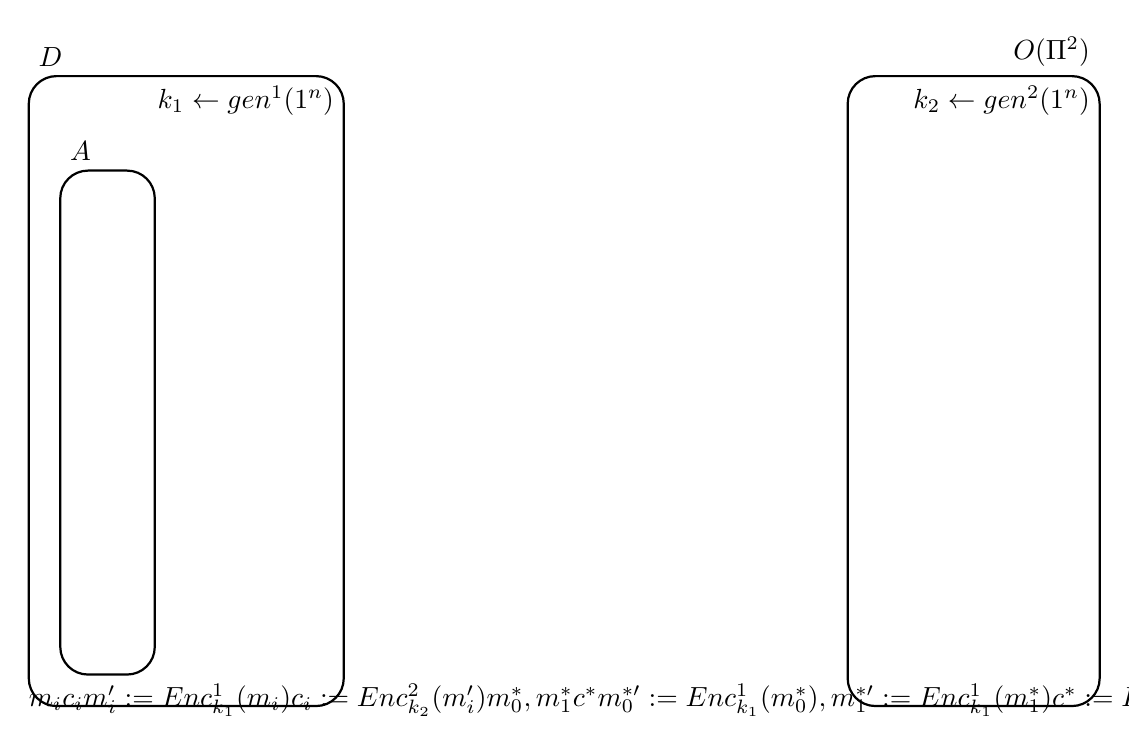
\begin{tikzpicture}[scale=0.8]
			%structure
			\draw[rounded corners=10pt,thick] (0,0) rectangle (5,10);
			\draw[rounded corners=10pt,thick] (0.5,0.5) rectangle (2,8.5);
			\draw[rounded corners=10pt,thick] (13,0) rectangle (17,10);
			\node[above right] at (0,10) {$D$};
			\node[above right] at (0.5,8.5) {$A$};
			\node[above left] at (17,10) {$O(\Pi^2)$};
			\node[below left] at (5,10) {$k_1 \leftarrow gen^1(1^n)$};
			\node[below left] at (17,10) {$k_2 \leftarrow gen^2(1^n)$};
			
			%train phase
			\flect (2,8) -- (4,8) \mess {$m_i$};
			\flect (4,7) -- (2,7) \mess {$c_i$};
			\flect (5,8) -- (13,8) \mess {$m_i':=Enc_{k_1}^1(m_i)$};
			\flect (13,7) -- (5,7) \mess {$c_i:=Enc_{k_2}^2(m_i')$};
			
			%challenge phase
			\flecc (2,5.5) -- (4,5.5) \mess {$m^{\ast}_0,m^{\ast}_1$};
			\flecc (4,4.5) -- (2,4.5) \mess {$c^\ast$};
			\flecc (5,5.5) -- (13,5.5) \mess {$m
			_0^{\ast\prime}:=Enc_{k_1}^{1}(m_0^\ast),m_1^{\ast\prime}:=Enc_{k_1}^{1}(m_1^{\ast})$};
			\flecc (13,4.5) -- (5,4.5) \mess {$c^\ast:=Enc_{k_2}^{2}(m_b^{\ast\prime})$};
			\node[below right] at (13,5.5) {$b \leftarrow \{0,1\}$};
			
			%train phase
			\flect (2,3) -- (4,3) \mess {$m_i$};
			\flect (4,2) -- (2,2) \mess {$c_i$};
			\flect (5,3) -- (13,3) \mess {$m_i':=Enc_{k_1}^1(m_i)$};
			\flect (13,2) -- (5,2) \mess {$c_i:=Enc_{k_2}^2(m_i')$};
			
			% output
			\flec (2,1) -- (3,1) node[pos=1,right] {$b'$};
			\flec (5,1) -- (6,1) node[pos=1,right] {$b''=b'$};
		\end{tikzpicture}
	\end{center}
	As we can see in every case, the distinguisher will have the same probability to find the message encrypted by the oracle than the attacker to break the scheme. As the attacker can only have a probability of $1/2 + \varepsilon$ to succeed the distinguisher will have the same probability. So, the scheme $\Pi$ is secure.
	
	\item As seen in the previous development, if $\Pi^2$ is CPA secure, $\Pi$ is CPA secure. There is no restriction on $\Pi^1$ in that case. Therefore $\Pi^1$ could be such that $Enc^1_{k_1}(m):=m$ which is obviously not CPA secure. So the proposition is false.
	
	\item Idem
	
	\item \textbf{If $\Pi^1$ is CPA secure, is it $\Pi'$ CPA secure?}\\
	The $\Pi'$ scheme is CPA secure if and only if $\Pi^2$ is also CPA secure.
	
	For example, if $Enc_{k_2}^2(m) = m$ then the scheme $\Pi'$ is not CPA secure.
	
	TO DEVELOP. (solution of the teaching assistant?)
	
	\item TODO
	
	\item TODO
	
	\item TODO
\end{enumerate}

\end{solution}

